\documentclass[10pt]{beamer}

\usetheme{metropolis}
\usepackage{appendixnumberbeamer}

\usepackage{booktabs}
\usepackage[scale=2]{ccicons}

\usepackage{pgfplots}
\usepgfplotslibrary{dateplot}

\usepackage[brazil]{babel}
\usepackage{multicol}


\usepackage{xspace}
\newcommand{\themename}{\textbf{\textsc{metropolis}}\xspace}

\title{Realoque}
\subtitle{``Conectando quem tem a quem precisa''}
\date{\today}
\author{Eduardo G. S. Cardoso \and Igor M. S. Moreira \and João V. da S. D. Canavarro}
\institute{Hackaton SERPRO}
\titlegraphic{\hfill
\includegraphics[height=2.5cm]{demo/images/bg-hackathon-normal.png}}

\begin{document}

\maketitle

\begin{frame}{Agenda}
  \setbeamertemplate{section in toc}[sections numbered]
  \tableofcontents[]
\end{frame}

\section{Introdução}

\begin{frame}[fragile]{A ideia}

    \begin{quote}
        Para proprietários de imóveis ociosos -- sobretudo o governo -- que necessitam de uma forma transparente e eficiente de anúncio de aluguel ou venda deles a entes privados nele interessados, o \textbf{Realoque} é uma tecnologia \textit{web} de aproximação que visa reduzir a complexidade  e burocracia desse tipo de comércio. Ele se diferencia do mero uso dos bancos de dados disponibilizados pelo governo atualmente ao tratar e unificar dados de diversas fontes em uma interface acessível.
    \end{quote}
    
\end{frame}

\begin{frame}[fragile]{Contextualização}

    O patrimônio imobiliário da união é \textbf{grande}.
    
    \begin{figure}
        \centering
        \caption{655 mil imóveis, administrados em \textit{databases} inconsistentes}
        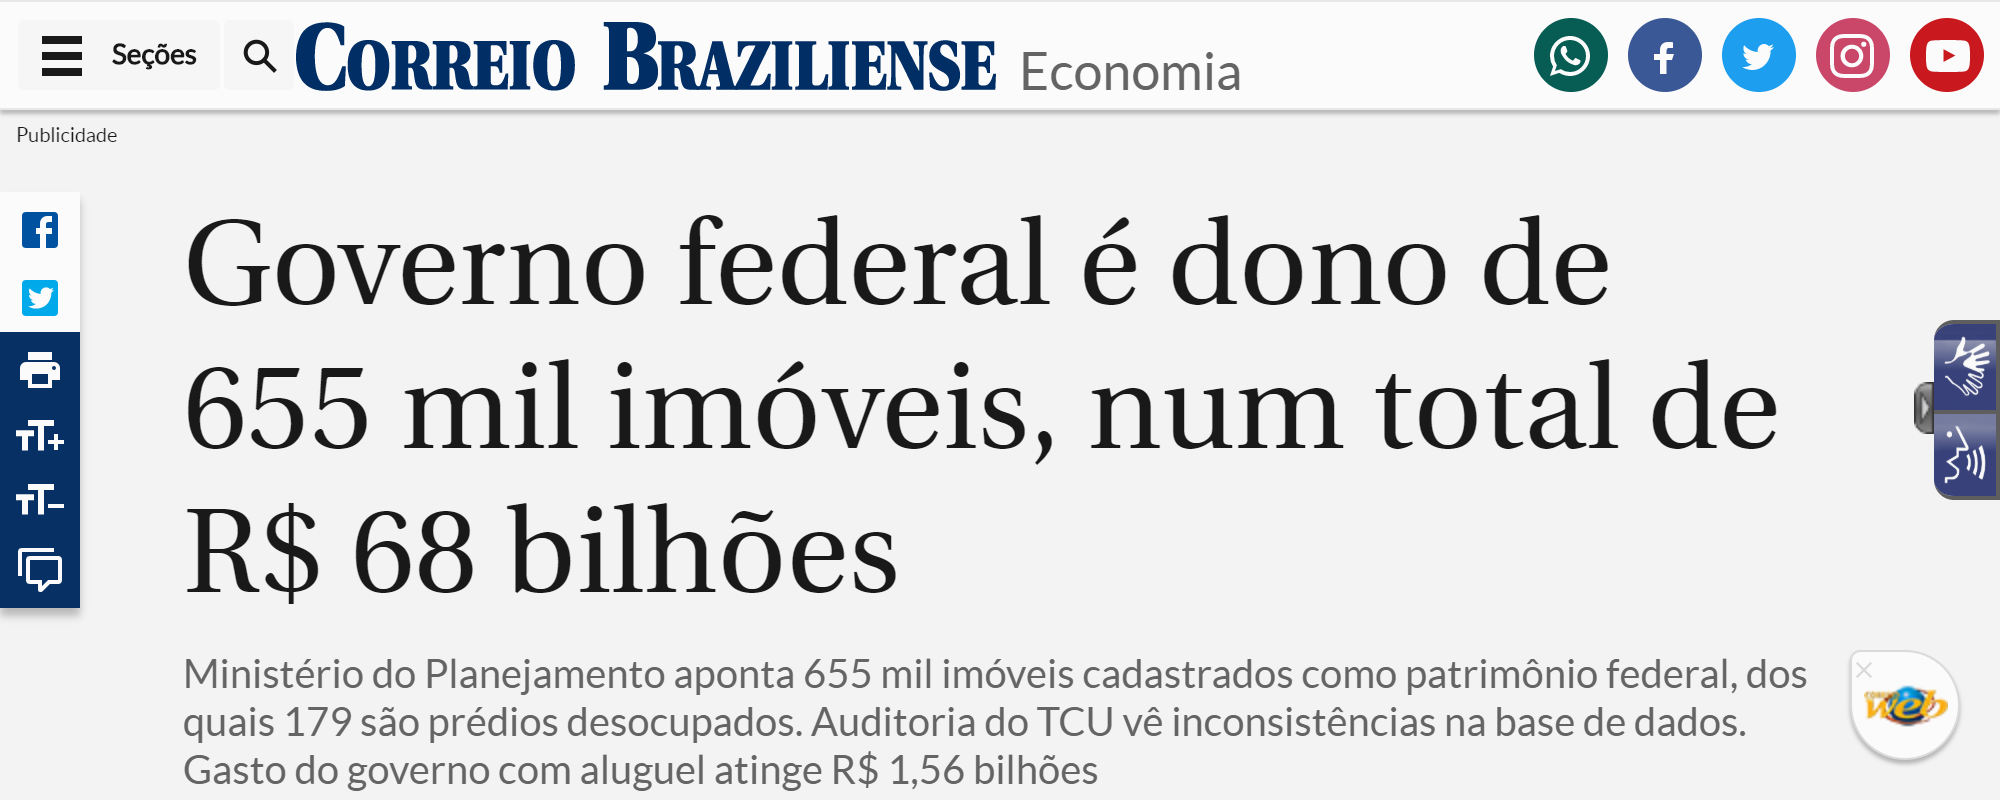
\includegraphics[width=\linewidth]{demo/images/noticia11_multiply.png}
        \legend{\textbf{Fonte:} Correio Braziliense}
        \label{fig:noticia1}
    \end{figure}
    
\end{frame}

\begin{frame}[fragile]{Contextualização}

    O patrimônio imobiliário da união é \textbf{grande}. \textbf{Muito grande}.
    
    \begin{figure}
        \centering
        \caption{notícia do InfoMoney}
        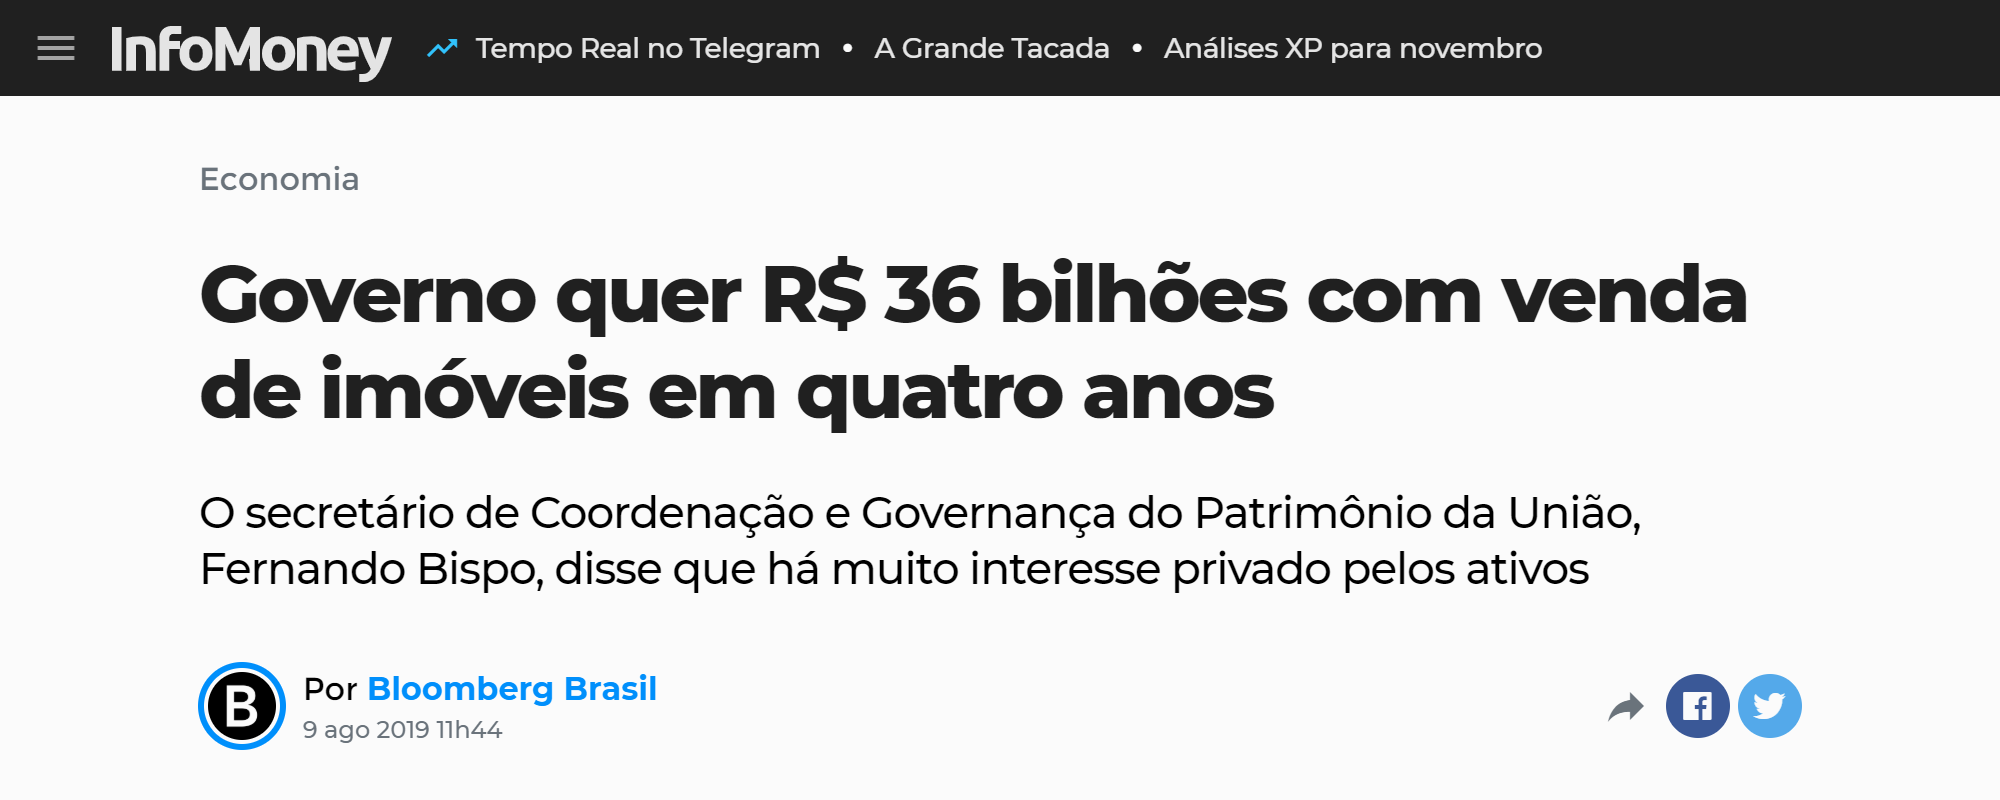
\includegraphics[width=\linewidth]{demo/images/noticia2_multiply.png}
        \legend{\textbf{Fonte:} InfoMoney}
        \label{fig:noticia2}
    \end{figure}
    
\end{frame}

\begin{frame}[fragile]{Contextualização}
    
    \begin{figure}
        \centering
        \caption{$4.000$ imóveis valem metade do valor dos demais $651.000$ imóveis?}
        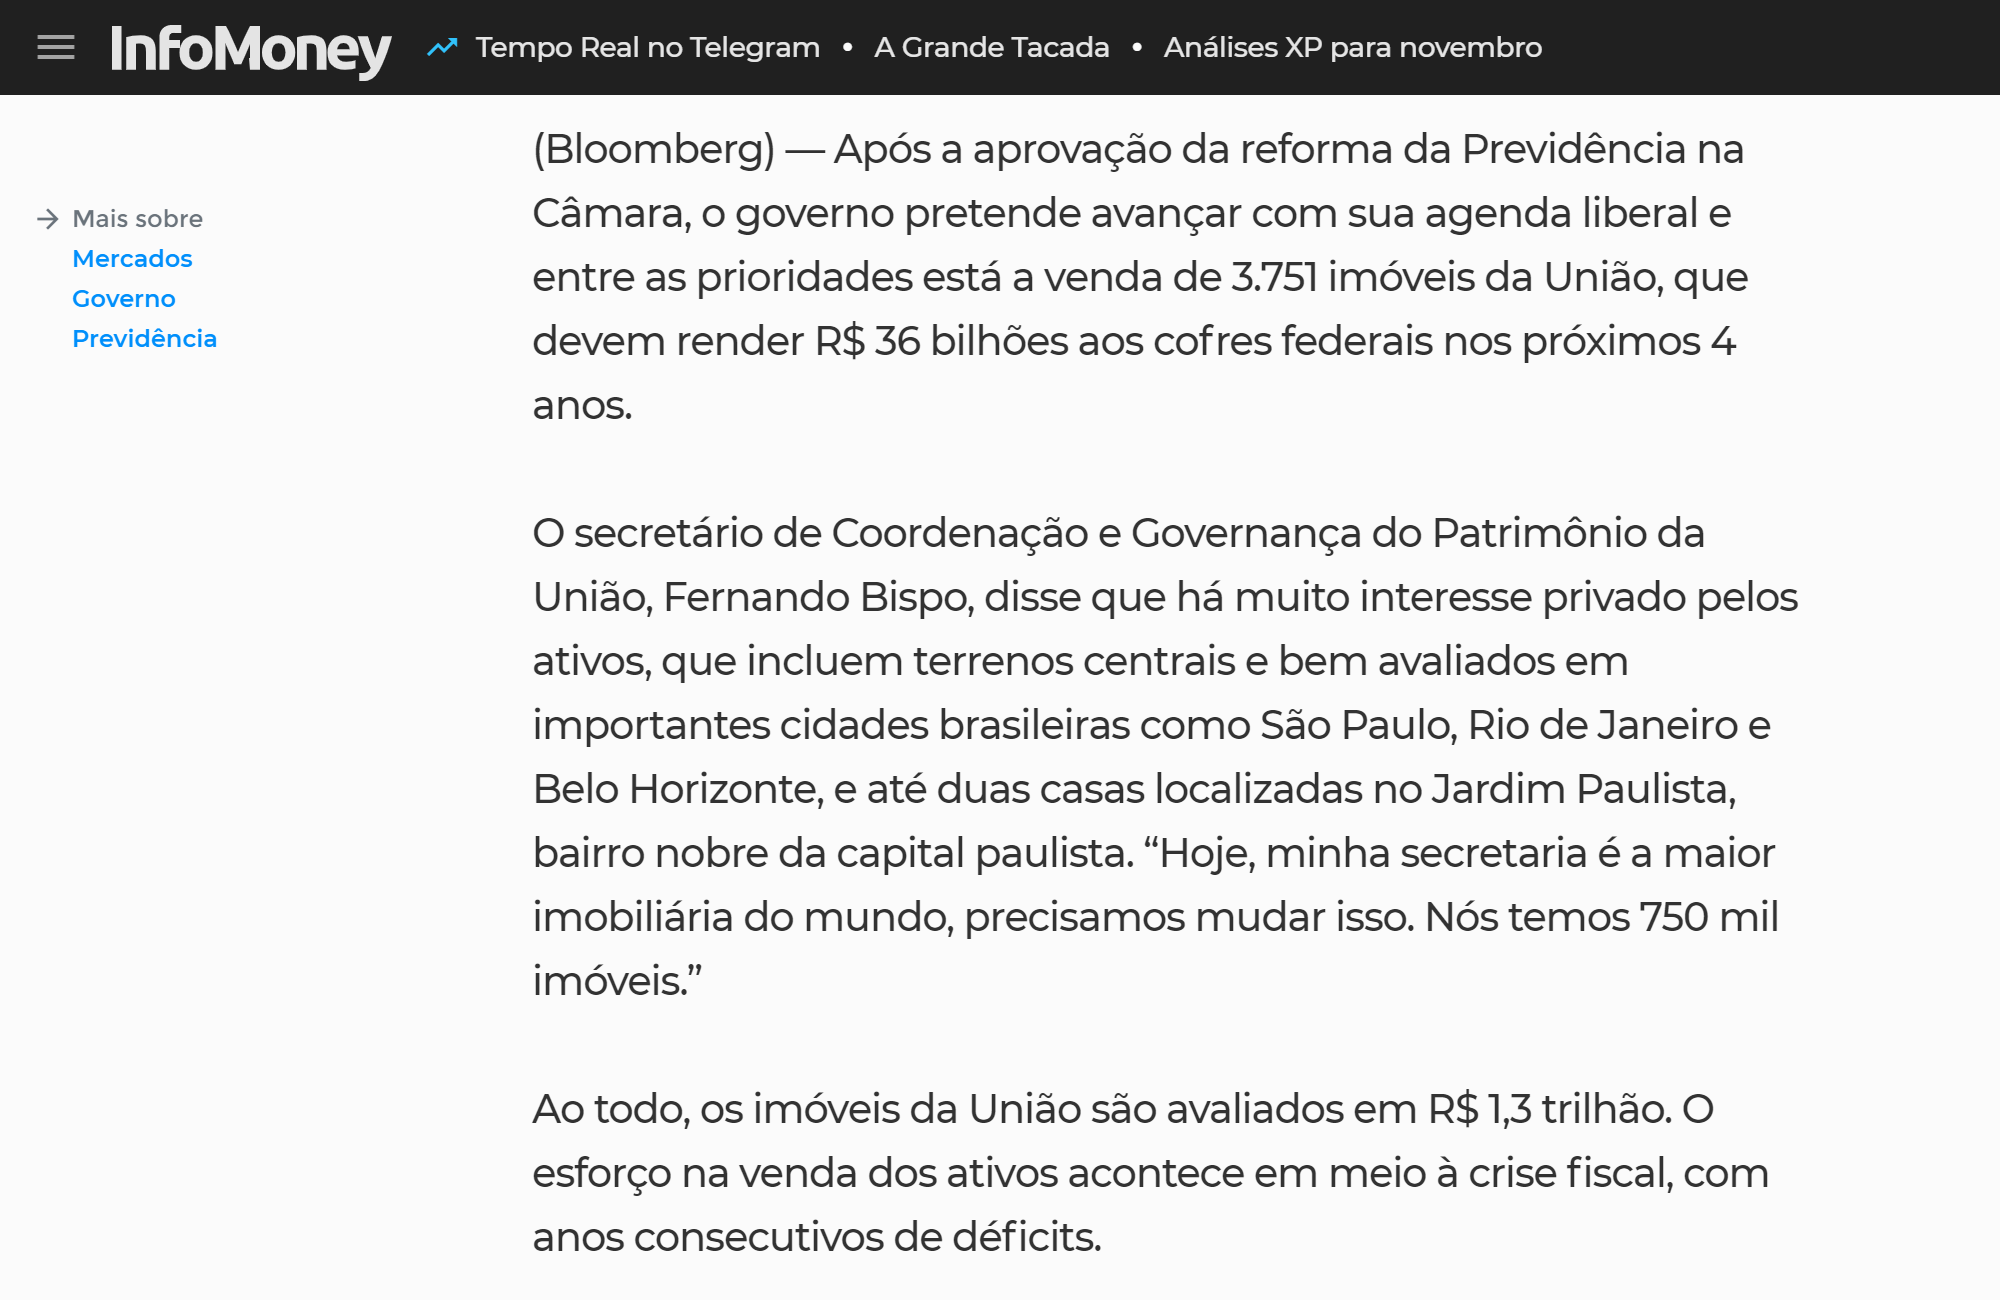
\includegraphics[width=\linewidth]{demo/images/noticia2_conteudo2_multiply.png}
        \label{fig:noticia2}
    \end{figure}
    
\end{frame}

\begin{frame}[fragile]{Contextualização}

    Quantificar esse portfólio \textbf{não é tarefa trivial}. E o governo \textbf{sabe que está deixando a desejar}.
    
    \begin{figure}
        \centering
        \caption{quadro atual de gestão patrimonial da União}
        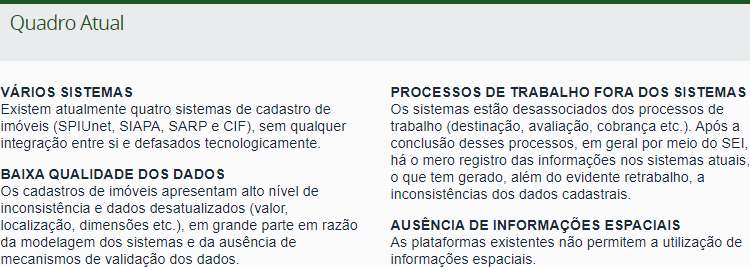
\includegraphics[width=\linewidth]{demo/images/planejamento_sistema_multiply.png}
        \legend{\textbf{Fonte:} Ministério da Economia}
        \label{fig:noticia2}
    \end{figure}
    
\end{frame}

\begin{frame}[standout]
  Se a gestão patrimonial não é transparente nem para o governo, o que dizer dela na perspectiva do cidadão?
\end{frame}

\begin{frame}{Propósito}
    É público e notório que:
    
    \begin{itemize}
        \item<+-> Os governos em geral possuem \textbf{patrimônio ocioso} ou sub-utilizado que poderia ser concedido ou vendido a entes privados;
        \item<+-> Empresas (governamentais ou não) e corretoras estão sempre à procura de \textbf{instalações adequadas} aos seus propósitos.
    \end{itemize}
    
	nossa solução busca aproximar esses dois pontos.
\end{frame}

\begin{frame}[fragile]{Justificativa}

    \textbf{A economia imobiliária} -- seja para uso residencial, seja para uso comercial -- \textbf{mudou muito} nos últimos anos.
    
    \begin{figure}
        \centering
        \caption{evolução da economia imobiliária}
        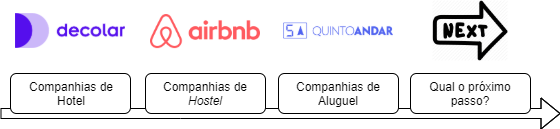
\includegraphics[width=\linewidth]{demo/images/evolucao_imobiliaria.png}
        \legend{\textbf{Fonte:} Acervo Próprio}
        \label{fig:noticia2}
    \end{figure}
    
    \begin{block}{O mercado imobiliário está mais dinâmico do que nunca.}
        \alert{Mas acreditamos que há o que melhorar.}
    \end{block}
    
\end{frame}

\begin{frame}[standout]
  \begin{center}
      Introduzindo a
      
      
\includegraphics[height=.1\linewidth]{demo/images/realoque.png}
  \end{center}
\end{frame}

\section{O produto}

\begin{frame}{Visão geral}
    Uma plataforma especializada para intermediar a venda e aluguel de imóveis de forma transparente, simplificada, eficiente e segura que busca atender a:
    
    \begin{itemize}
        \item<+-> \textbf{Governos:} tem-se uma alternativa para a divulgação transparente, ampla e efetiva do interesse governamental em alugar ou desfazer-se de imóveis;
        \item<+-> \textbf{Empresários e corretoras:} estes últimos, sobretudo, podem interessar-se pelos órgãos da União, geralmente bem localizados, ou pelo potencial de divulgação do site; e
        \item<+-> \textbf{Consumidores em geral:} eventualmente, ter-se-ia um sistema equivalente à OLX para imóveis, mas com segurança aprimorada,
    \end{itemize}
    
	buscando sempre abstrair a burocracia inerente a esse tipo de transação.
\end{frame}

\section{O \textit{Minimum Viable Product}}

\begin{frame}{Tecnologias utilizadas}
    \begin{multicols}{4}
        \begin{figure}
            \centering
            
\includegraphics[width=\linewidth]{demo/images/python.png}
            \label{fig:python}
        \end{figure}
        \begin{figure}
            \centering
            
            \hfill
            
            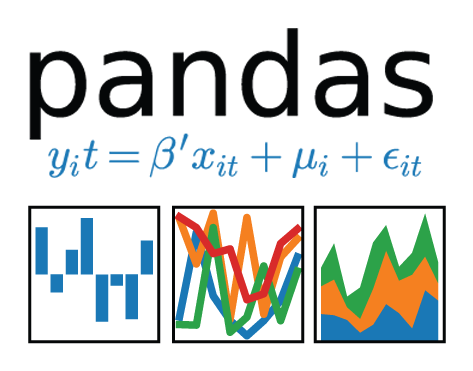
\includegraphics[width=\linewidth]{demo/images/pandas.png}
            \label{fig:pandas}
        \end{figure}
        \begin{figure}
            \centering
            
\includegraphics[width=\linewidth]{demo/images/flask.png}
            \label{fig:python}
        \end{figure}
        \begin{figure}
            \centering
            \vspace*{-.3cm}
            
\includegraphics[width=\linewidth]{demo/images/sqlalchemy.png}
            \label{fig:python}
        \end{figure}
    \end{multicols}
    \begin{multicols}{3}
        \begin{figure}
            \centering
            
            \hfill
            
            
\includegraphics[width=\linewidth]{demo/images/php.png}
            \label{fig:python}
        \end{figure}
        \begin{figure}
            \centering
            
            \hfill
            
            
\includegraphics[width=\linewidth]{demo/images/codeigniter.png}
            \label{fig:pandas}
        \end{figure}
        \begin{figure}
            \centering
            
\includegraphics[width=\linewidth]{demo/images/postgresql.png}
            \label{fig:python}
        \end{figure}
    \end{multicols}
\end{frame}

\begin{frame}{Bases de Dados Utilizadas}
    \begin{itemize}
        \item<+-> \textbf{Imóveis da União (SIAPA):} \textit{dataset} com informações sobre as moradias e terrenos que pertencem ao governo;
        \item<+-> \textbf{IPTU (Prefeitura de São Paulo):} \textit{dataset} utilizado para estimativas de preço dos imóveis da união.
    \end{itemize}
\end{frame}

\begin{frame}[standout]
  \begin{center}
      Vamos à demonstração!
  \end{center}
\end{frame}

\begin{frame}{Perspectivas futuras}
    \begin{itemize}
        \item<+-> \textbf{Expandir o leque de métricas utilizadas}, mediante colaboração com os órgãos envolvidos (cartórios, corretores, dados obtidos com o uso da plataforma, entre outros);
        \item<+-> Mediante a ampliação dos dados, \textbf{estabelecer um fluxo de alimentação de algoritmos de aprendizado de máquina} para a previsão de aspectos como o preço, por exemplo;
        \item<+-> \textbf{Prover mais visualizações}, a fim de ajudar o usuário a tomar decisões mais rapidamente;
        \item<+-> \textbf{Implementar a parte restrita ao usuário}, para registro de interesses e oferta personalizada de imóveis.
    \end{itemize}
\end{frame}

\begin{frame}[standout]
    Obrigado pela atenção! Dúvidas?
\end{frame}

\end{document}
